\documentclass[12pt]{article}
\usepackage[utf8]{inputenc}
\usepackage[brazil]{babel}
\usepackage[margin = 1in]{geometry}
\usepackage{graphicx}
\usepackage{subfigure}
\usepackage{minted}
\usepackage{indentfirst}
\usepackage{float}
\usepackage{multirow}


\begin{document}

    
\begin{titlepage}
 \vfill
  \begin{center}
   {\large \textbf{UNIVERSIDADE FEDERAL DO PARANÁ \\ SETOR DE TECNOLOGIA \\ DEPARTAMENTO DE ENGENHARIA ELÉTRICA}} \\[5cm]

  {\large {Marco Antonio Rios  GRR20133243 \\ Wendeurick Silverio GRR20134722} }\\[4cm]


   {\Large \textbf{Projetos de Sistemas Digitais em PLD - TE087} \\ Laboratório 6}\\[6cm]
    \vfill

    \vspace{2cm}

    \large \textbf{Curitiba}

    \large \textbf{\today}

      \end{center}
\end{titlepage}

\clearpage
%\tableofcontents    
%\clearpage

\section{Desafio 1}
O primeiro desafio propõe um decodificador para \emph{display} de 7 segmentos, cuja entrada é um valor inteiro e a saída é um vetor \emph{std\_logic} correspondente aos respectivos segmentos a serem acesos/apagados conforme a entrada.

\subsection{Implementação}

Abaixo, o código \emph{VHDL} da implementação.

\inputminted{vhdl}{display7seg.vhd}

\clearpage

\section{Desafio 2}

O segundo desafio propõe um contador crescente (0 a 9) cujo valor deve ser apresentado em um dos \emph{displays} de 7 segmentos do kit Nexys2.

\subsection{Implementação}

Abaixo, o código \emph{VHDL} da implementação.

\inputminted{vhdl}{desafio1.vhd}

\subsection{Mapeamento das portas I/0}

Abaixo, o mapeamento das entradas e saídas para o kit Nexys2.

\inputminted{vhdl}{desafio1_pins.ucf}

\subsection{Simulação}

Abaixo, o código \emph{VHDL} do Testbench.

\inputminted{vhdl}{tb_desafio1.vhd}

\begin{figure}[!h]
    \centering
    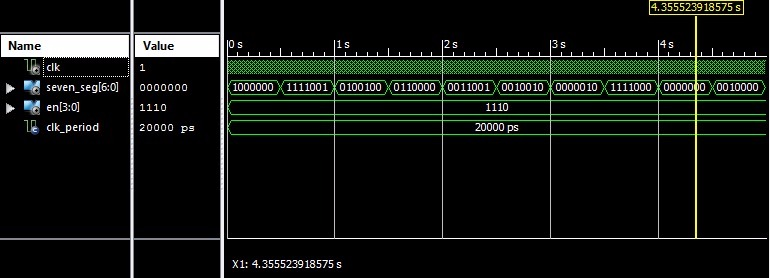
\includegraphics[width=1.0\textwidth]{tb_desafio1.jpg}
    \caption{Testbench do Desafio 2.}
\end{figure}

\end{document}
